\documentclass{article}

% if you need to pass options to natbib, use, e.g.:
% \PassOptionsToPackage{numbers, compress}{natbib}
% before loading nips_2016
%
% to avoid loading the natbib package, add option nonatbib:
% \usepackage[nonatbib]{nips_2016}

\usepackage[final, nonatbib]{nips_2016}

% to compile a camera-ready version, add the [final] option, e.g.:
%\usepackage[final]{nips_2016}

\usepackage[utf8]{inputenc} % allow utf-8 input
\usepackage[T1]{fontenc}    % use 8-bit T1 fonts
\usepackage{hyperref}       % hyperlinks
\usepackage{url}            % simple URL typesetting
\usepackage{booktabs}       % professional-quality tables
\usepackage{amsfonts}       % blackboard math symbols
\usepackage{nicefrac}       % compact symbols for 1/2, etc.
\usepackage{microtype}      % microtypography

% My packages
\usepackage{amsmath}        %Matrix
\usepackage{graphicx}       %Graphics
\usepackage{subcaption}     %Subfigures


\title{Design Optimization of a Stochastic Multi-Objective Problem: \\Gaussian Process Regressions for Objective Surrogates}

% The \author macro works with any number of authors. There are two
% commands used to separate the names and addresses of multiple
% authors: \And and \AND.
%
% Using \And between authors leaves it to LaTeX to determine where to
% break the lines. Using \AND forces a line break at that point. So,
% if LaTeX puts 3 of 4 authors names on the first line, and the last
% on the second line, try using \AND instead of \And before the third
% author name.

\author{
  Juan S. Martinez\\
  Department of Electrical and Electronic Engineering\\
  Universidad de los Andes\\
  Bogotá, Colombia \\
  \texttt{js.martinez777@uniandes.edu.co} \\
  %% examples of more authors
  %% \And
  %% Coauthor \\
  %% Affiliation \\
  %% Address \\
  %% \texttt{email} \\
  %% \AND
  %% Coauthor \\
  %% Affiliation \\
  %% Address \\
  %% \texttt{email} \\
  %% \And
  %% Coauthor \\
  %% Affiliation \\
  %% Address \\
  %% \texttt{email} \\
  %% \And
  %% Coauthor \\
  %% Affiliation \\
  %% Address \\
  %% \texttt{email} \\
}

\begin{document}
% \nipsfinalcopy is no longer used

\maketitle

\begin{abstract}
    Global optimization of expensive, multi-modal and noisy multi-objective functions is a common problem that comes up frequently in various areas of computational and experimental research. Along with being expensive to evaluate and noisy, we are also particularly interested in cases where the objective function under consideration is a black box and does not provide gradient information of the quantity of interest (QoI) w.r.t to the inputs. Because of the high cost of every single evaluation of such objective functions, we can only obtain a limited number of evaluations. This necessarily induces epistemic uncertainty (lack of knowledge due to limited data) on our problem. The Bayesian approach provides a natural framework to approach this problem, building Gaussian process surrogates that model the objective functions and allow a sequential optimization process. The method applies the expected improvement (EI) information acquisition function in each iteration to perform an efficient global optimization (EGO) and discover the Pareto front of the problem, which contains the set of optimal solutions of the objectives. We implemented this method in a NanoHUB tool and tested it with synthetic examples and real observations of an expensive experiment, where it proved to be efficient in finding the corresponding set of optimal solutions for each problem. This methodology demonstrates how the efficiency of the Bayesian approach for handling epistemic uncertainty in multi-objective optimization problems, dealing with limited observations and avoiding a high amount of evaluations of time-consuming codes or expensive experiments.
\end{abstract}

\section{Introduction}

A great variety of problems in science and engineering can be expressed as optimization problems, where a function that describes the operation of a system should be minimized or maximized, restricted to some constraints imposed by the system itself. For example, a supermarket may want to minimize its inventory purchases while keeping enough stock for its operation, or in a metal-forming shop, a manufacturer may want to maximize the performance of the manufacturing system adjusting certain parameters, like the forming temperature and the die geometry \cite{Huang2006}. Moreover, real optimization problems do not have trivial or "easy" solutions, since in many cases the optimization could target: black-box systems where the physics and mathematics of the process are not well known; expensive simulations or evaluations of objective functions \cite{Jones1998}; introduction of uncertainty at the output due to noise in the input data; and multiple objectives. In this context, a need for the design of a method for solving stochastic multi-objective optimization problems arises and becomes important in the science and engineering community.\\

One of the first issues in optimization that arises in real science and engineering problems is the lack of knowledge of the physics that rules the underlying process of the system being studied. This case is treated as a black-box system where limited output observations are available to build a model that could describe the system with the highest accuracy possible. Optimization under these circumstances has been approached from different perspectives, for example, advances in efficient global optimization of expensive simulations have been made through the analysis of various criteria of the problem, like the expected improvement (EI) of running the simulation at a particular point; also, stopping criteria for the sequential optimization processes that rules black-box problems have also been developed \cite{Jones1998}, as well as curiosity-driven techniques \cite{Schaul2011}. In this matter, the structure for solving black-box optimization problems is based on building response surfaces over observed data. The taxonomy of this process includes the use of different criteria to evaluate the sequential process of optimization, in which the EI information acquisition scheme has proven to be more efficient than the other criteria, such as the probability of improvement and lower and upper confidence bounds \cite{Jones2001}.\\

This study shows how black-box systems have been approached in order to perform a sequential process of optimization. However, dealing with a black-box system is only one of the many problems optimization faces in real scientific and engineering scenarios. Another major issue corresponds to the effect of epistemic uncertainty, noise in the input data, and how it propagates in the surrogate models used in optimization. For this problem, the use of Gaussian process regression has become a very useful and effective strategy to generate a stochastic approach for the problem \cite{Wang2016}, modifying the EI criteria and considering Bayesian models to manipulate efficient global optimization schemes, as presented in \cite{Huang2006}, \cite{Pandita2016} and \cite{Li2014}. Stochastic approaches to optimization problems often require the development and implementation of probabilistic machine learning techniques, which are fully developed tools as documented by Seeger \cite{Seeger2004} and Davidson-Pilon \cite{Davidson-Pilon2014}. Although developed tools and models for optimization form the state of the art of stochastic optimization, other great issue arises in the systems studied so far, which is the problem of targeting multiple objectives inside the same system.\\

Multi-objective optimization (MOO) problems are widely studied through different techniques, which include the application of genetic algorithms through the appliance of evolutionary strategies \cite{Costa2006}. In MOO problems, genetic algorithms are used to obtain the Pareto front, which contains the optimal solutions to the problem studied and it is typically the main objective of these type of algorithms, but also, evolutionary techniques have been developed to solve expensive simulation-based optimization problems as presented in \cite{Guo2007} and \cite{Huang2009}. Although these techniques address MOO problems, they do not consider an stochastic approach to handle uncertainty. On the other hand, this type of considerations have been made, and they show how MOO problems can be addressed by an extension of the expected improvement (EI) criteria, deriving a closed form of the information acquisition function \cite{wagner2010expected}. Within this context, the study presented here aims to develop a "greedy" and reliable method for MOO problems for real black-box systems, addressing uncertainty propagation and considering expensive objective function evaluations through Gaussian process regression surrogates.\\

The method relies on Gaussian process regressions to build surrogates for the objective functions of the system, as an approximation of the functions that map the inputs to the corresponding outputs. This surrogates are able to consider uncertainty at the input and enables the addition of observations to enrich prior beliefs of the problem, in order to adjust the response surfaces and obtain a better description of the system. Section 2 describes the methodology of these regressions and section 3 presents the results of the sequential optimization process using the surrogates. Section 4 discusses the results obtained for the synthetic example and the real test example and section 5 presents the conclusions of this work.

\section{Methodology}

The MOO problem of black-box systems was addressed through a Bayesian approach, where initial observations of the experiments we want to model provide information that enrich prior beliefs and help us determine better surrogates for our objectives. As only limited information is available, Gaussian process regression was used as a technique for building the functions, this method is able to quantify the epistemic uncertainty induced by the reduced amount of observations.

A Gaussian process (GP) is a collection of random variables, any finite number of which have a joint Gaussian distribution\cite{Seeger2004}. It represents a generalization of a multivariate Gaussian distribution to infinite dimensions, over a space of functions. A GP is defined by its mean function $m(\vec{x})$ and covariance function $k(\vec{x},\vec{x}')$; they are defined for a process $f(\vec{x})$ as:

\begin{equation}
    m(\vec{x}) = \mathbb{E}[f(\vec{x})],
\end{equation}
\begin{equation}
    k(\vec{x},\vec{x}') = \mathbb{E}[(f(\vec{x})-m(\vec{x}))(f(\vec{x}')-m(\vec{x}'))].
\end{equation}

Then, the process is defined as a Gaussian process as: \cite{Seeger2004}

\begin{equation}
    f(\vec{x}) \sim GP(m(\vec{x}), k(\vec{x},\vec{x}')).
\end{equation}

In a more general case, the mean and covariance functions depend on a set of \textit{hyperparameters} denoted by $\vec{\theta}$. Taking this into account, a Gaussian process could be defined as:

\begin{equation}
    f(\cdot)|\vec{\theta} \sim GP(f(\cdot)|m(\cdot;\vec{\theta}),k(\cdot,\cdot;\vec{\theta})).
\end{equation}

As for the Bayesian approach taken in this study, a GP was used to model our prior beliefs about the objective functions in the system. In this case, all information about the mean can be included in the covariance function. Thus, $m(\cdot;\vec{\theta})$ was taken to be zero. On the other hand, the covariance function used was the squared exponential (SE) covariance:

\begin{equation}
    k(\vec{x},\vec{x}';\vec{\theta}) = s^2 \exp \left \{ -\frac{1}{2}\sum_{i=1}^{d}\frac{(x_i - x_i')^2}{\ell_i^2} \right \},
\end{equation}

where $d$ is the dimensionality of the input space, $s > 0$ is the signal strength of the response and $\ell_i > 0$ is the lengthscale along the input dimension $i$. For this case, the set of hyperparameters $\vec{\theta}$ is composed as $\vec{\theta} = \{s, \ell_1, \ldots, \ell_d\}$. This design for the mean function and the covariance function is the same as the approach taken in \cite{Pandita2016}.\\

In the Gaussian process regression, noisy and limited observations provide a likelihood of the data subject to the hyperparameters of the model. Assuming a Gaussian noise with unknown variance $\sigma^2$, the likelihood is\cite{Pandita2016}:

\begin{equation}
    p(\vec{y}_{1:n}|\vec{x}_{1:n}, \vec{\psi}) = \mathcal{N}(\vec{y}_{1:n}|\vec{f}_{1:n},\textbf{K}_n(\vec{\theta}) + \sigma^2\textbf{I}_n).
    \label{likelihood}
\end{equation}

As expressed in equation \ref{likelihood}, the likelihood has the PDF of a multivariate normal random variable with mean $\vec{f}_{1:n}$ and covariance matrix $\textbf{K}_n(\vec{\theta}) + \sigma^2\textbf{I}_n$, where $\textbf{I}_n \in \mathbb{R}^{n\times n}$ is the identity matrix, $\vec{\psi} = \{ \vec{\theta}, \sigma \} $ and $\textbf{K}_n \in \mathbb{R}^{n\times n}$ is the covariance matrix of the form:

\begin{equation}
    \textbf{K}_n(\vec{\theta}) =
    \begin{bmatrix}
        k(\vec{x}_1,\vec{x}_1;\vec{\theta}) & \cdots & k(\vec{x}_1,\vec{x}_n;\vec{\theta}) \\
        \vdots & \ddots & \vdots\\
        k(\vec{x}_n,\vec{x}_1;\vec{\theta}) & \cdots & k(\vec{x}_n,\vec{x}_n;\vec{\theta})
    \end{bmatrix}.
\end{equation}

Through Bayes rule, combining the prior beliefs and the likelihood of observed data produces a posterior distribution of the function space that represents our model. This distribution is described as\cite{Pandita2016}:

\begin{equation}
    p(f(\cdot)|\vec{x}_{1:n},\vec{y}_{1:n},\vec{\psi}) = GP(f(\cdot)|m_n(\vec{x};\vec{\psi}),k_n(\vec{x},\vec{x}';\vec{\psi})),
\end{equation}

where $m_n(\vec{x};\vec{\psi})$ and $k_n(\vec{x},\vec{x}';\vec{\psi})$ are the posterior mean and covariance functions, their analytical expressions can be found in \cite{Pandita2016}. With this in mind, the common procedure to adjust the posterior model is to maximize the logarithm of the likelihood\footnote{Maximizing the likelihood often requires unachievable computational resources, instead, the logarithm of the function has the same behavior and it demands more reasonable computation requirements}, which produces the corresponding hyperparameters that optimize the model.\\

To illustrate this, figure \ref{gp_regression} shows a Gaussian process regression for a cosine function with Gaussian noise added, the regression was built with a signal strength of 1 and a lengthscale of 1 for the 1-dimensional input. The black "X" marks represent sample points of the real function and the blue line represents the mean function of the sampled regression, along with the shaded area that represents the uncertainty of the surrogate. In figure \ref{gp}, only prior information is used to build the regression, but on figure \ref{gp_optimized}, observed data is applied and the posterior is adjusted due to the maximization of the likelihood of data. As we can see, uncertainty is reduced around the observed data but increases around isolated data points or where there are no observations.

\begin{figure}
\centering
	\begin{subfigure}[b]{0.4\textwidth}
        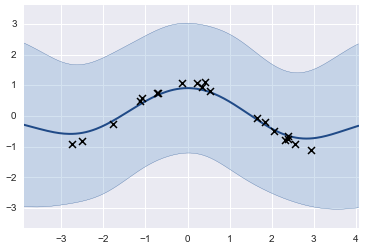
\includegraphics[width=\textwidth]{gp_cosine.png}
        \caption{Gaussian process regression}
        \label{gp}
	\end{subfigure}

	\begin{subfigure}[b]{0.4\textwidth}
        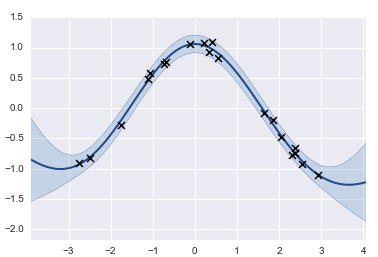
\includegraphics[width=\textwidth]{gp_cosine_optimized.png}
	    \caption{Optimized Gaussian process regression}
	    \label{gp_optimized}
	\end{subfigure}
\caption{Gaussian process regression of cosine function}
\label{gp_regression}
\end{figure}

This methodology applies for a single objective but can be extended to multiple outputs, and a sequential optimization algorithm for multi-objective problems can be implemented. This is the case for the overall project, where a sequential algorithm uses an extension of the expected improvement (EI) as the best information acquisition function (IAF)\cite{Jones2001} (applied to multiple objectives \cite{wagner2010expected}) to generate new evaluations of the experiment that is being modeled.

\section{Numerical Results}

\section{Discussion}

\section{Conclusions}

\bibliographystyle{ieeetr}
\bibliography{SURF_2016}

\section{Mentor Check}
\end{document}
